
\label{sec:disipadores}
\begin{figure}[H]
    \centering
    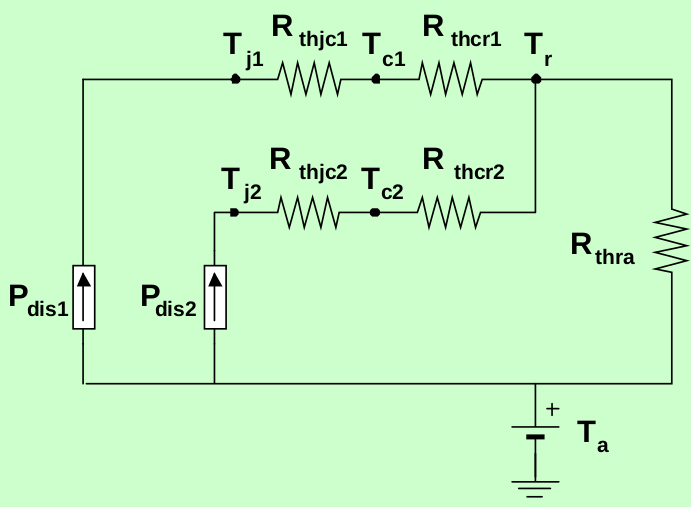
\includegraphics[height=0.4\textwidth]{img/calculo_disipador.png}
    \caption{Modelo térmico estacionario.}
    \label{fig:disipadores}
\end{figure}

En el peor caso, los transistores de potencia \textbf{2SC5200} de la etapa de salida y su par complementario \textbf{2SA1943} disipan cada uno $18 \si[per-mode=symbol]{\watt}$, ya que los mismos se utilizan en paralelo.

\begin{equation*}
T_r = R_{thra} * (P_{dis1}+P_{dis2}) + T_a
\end{equation*}

\begin{equation*}
T_r = T_{juntura_{N}} - (R_{t_{j-case}}+R_{t_{c-heat}})*P_{disN}
\end{equation*}

\begin{equation*}
T_r = 130 \si[per-mode=symbol]{\celsius} - (0.85 \si[per-mode=symbol]{\celsius\per\watt} + 0.1 \si[per-mode=symbol]{\celsius\per\watt})*(18*2 \si[per-mode=symbol]{\watt}) = 95.8 \si[per-mode=symbol]{\celsius}
\end{equation*}

\begin{equation*}
95.8 \si[per-mode=symbol]{\celsius} = R_{thra}*(18*2*2 \si[per-mode=symbol]{\watt}) + 40 \si[per-mode=symbol]{\celsius}
\end{equation*}

\begin{equation*}
R_{tha} = 0.77 \si[per-mode=symbol]{\celsius\per\watt}
\end{equation*}

En la  parte interna de la etapa de salida, tenemos que en el peor caso se disipan $3.25 \si[per-mode=symbol]{\watt}$ por cada transistor. Haciendo las mismas cuentas con otros valores.


\begin{equation*}
T_r = 120 \si[per-mode=symbol]{\celsius} - (6.25 \si[per-mode=symbol]{\celsius\per\watt} + 0.1 \si[per-mode=symbol]{\celsius\per\watt})*(3.25 \si[per-mode=symbol]{\watt}) = 99.36 \si[per-mode=symbol]{\celsius}
\end{equation*}

\begin{equation*}
R_{tha} = 9.13 \si[per-mode=symbol]{\celsius\per\watt}
\end{equation*}

\paragraph{Disipadores elegidos:}

Para la parte externa de la salida \textbf{ZD-23} $0.65 \si[per-mode=symbol]{\celsius\per\watt}$ , elegimos este modelo porque nos da un poco de margen.

\begin{figure}[H]
    \centering
    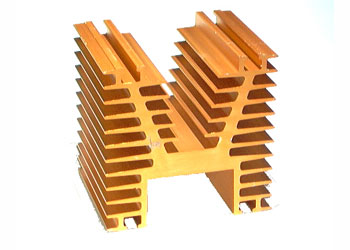
\includegraphics[height=0.4\textwidth]{img/zd23.jpg}
    \caption{Disipador \textbf{ZD-23}}
    \label{fig:diszd23}
\end{figure}


Para parte interna ZD-14 $2 \si[per-mode=symbol]{\celsius\per\watt}$, si bien solo necesitamos $9 \si[per-mode=symbol]{\celsius\per\watt}$ , elegimos este modelo porque nos da mas margen:

\begin{figure}[H]
    \centering
    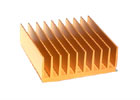
\includegraphics[height=0.4\textwidth]{img/zd14.jpg}
    \caption{Disipador \textbf{ZD-14}}
    \label{fig:diszd14}
\end{figure}